\documentclass[justified, nobib]{tufte-handout}

\usepackage{Haust2017verkefnablöð}

\title{Tölvunarfræði 1a  \semester - Námsáætlun og upplýsingar}

\begin{document}

\section{Námsáætlun}
\label{sec:schedule}

Námskeiðið er grundvallarnámskeið í tölvunarfræði og forritun, sérstaklega ætlað nemendum í vísindum og verkfræði.

\begin{marginfigure}
\caption{Merki Matlab}
\begin{center}

\includegraphics[width=0.5\linewidth]{matlab-logo}
\end{center}
\end{marginfigure}

Forritunarmálið sem notað verður í námskeiðinu er Matlab. Forritunarmálið og aðferðir sem því tengjast henta vel til vísindalegra útreikninga og gagnavinnslu.

\begin{table*}
\caption{Námsáætlun eftir vikum}
\label{tab:schedule}
\begin{center}
\renewcommand{\arraystretch}{1.2}
\begin{tabularx}{\linewidth}{lccXp{3cm}}
\toprule
&\multicolumn{2}{c}{Dagsetningar}&&\\
\cmidrule{2-3}
Vika&Þri&Fös&Námsefni&Kaflar\\
\midrule
1	&22/8	&25/8	& Kynning, Matlab-uppsetning, bitar og tvíundartölur, breytur, innbyggð föll, slembitölur &1.1 til 1.6\\
2	&29/8	&1/9	& Vigrar og fylki&2.1 til 2.5\\
3	&5/9	&8/9	& Reiknirit, skipanaskrár, inntak og úttak, einfaldar myndir&3.1 til 3.6\\
4	&12/9	&5/9	& Notendaskilgreind föll, stýrisetningar, röksegðir, \texttt{is}-föll&3.7, 4.1 til 4.6\\
5	&19/9	&-	    & For-lykkjur&5.1 til 5.2\\
6	&26/9	&29/9	& While-lykkjur, frekari vigurvinnsla, skipulag forrita, gildissvið breyta, aflúsun, kommutölur&5.3 til 5.5, 6.1, 6.2\\
7	&3/10	&6/10	& Gildissvið breyta, aflúsun. Strengir, aðgerðir á strengi&6.4, 6.5, 7.1 til 7.2\\
8	&10/10	&13/10	& Föll fyrir strengi, umbreytingar milli strengja og talna, hólfavigrar&7.3, 7.3, 8.1\\
9	&17/10	&20/10	& Færslur, skráarvinnsla&8.1, 9.1\\
10	&24/10	&27/10	& Frekari skráarvinnsla, MS Excel skrár, MAT-skrár&9.1 til 9.3\\
11	&31/11	&3/11	& Nafnlaus föll, fallshandföng, breytilegur fjöldi stika, hreiðruð föll, endurkvæm föll&10.1 til 10.5\\
12	&7/11	&10/11	& Öflugri teikniskipanir, hreyfimyndir, þrívíðar teikningar, teiknihandföng&11.1 til 11.7\\
13	&14/11	&17/11	& Tölfræðiföll, mengjaaðgerðir, röðun, helmingunarleit&12.1 til 12.3, 12.5\\
14	&21/11	&24/11	& Myndvinnsla, mátun ferils, samantekt&14.1\\
\bottomrule
\end{tabularx}
\end{center}
\end{table*}

\section{Kennari}
Aðalkennari er Eiríkur Ernir Þorsteinsson. Aðsetur er í Tæknigarði, 2. hæð, stofa 214. Sjá mynd \ref{fig:taeknigardur}.

\begin{marginfigure}
\caption{Önnur hæð í Tæknigarði. Kennara má finna í stofu 214.}
\label{fig:taeknigardur}
\begin{center}
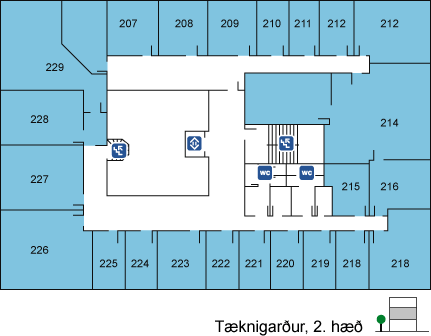
\includegraphics[width=\linewidth]{taeknigardur}
\end{center}
\end{marginfigure}

Til að hafa samband við kennara er ráðlagt að setja inn þráð á \href{piazza.com/hi.is/fall2017/tl105g/home}{Piazza}. Allar fyrirspurnir sem ekki fela í sér persónulegar upplýsingar ættu að fara þangað. Tölvupóstfang er \href{mailto:ernir@hi.is}{ernir@hi.is}.

\section{Tímar og námstilhögun}
Aðalkennsla fer fram í vikulegum fyrirlestrum. Fyrirlestrarnir eru á þriðjudögum klukkan 10 í HT-102 og föstudögum klukkan 11:40 í VRII-157.

Dæmatímar eru á mánudögum og þriðjudögum. Nemendum er frjálst að mæta í þá dæmatíma sem henta best.\footnote{Kennari mun skerast í leikinn ef sókn í dæmahópana verður mjög mismunandi.}

\subsection{Mætingaskylda}
Ekki er skylda að mæta í fyrirlestra eða dæmatíma (en sjá \nameref{sec:lecture-exercises}). Nemendur eru ábyrgir fyrir því að forgangsraða tíma sínum.
\subsection{Upptökur á fyrirlestrum}
Fyrirlestrar eru teknir upp þegar tæknin leyfir. Varað er við því að treysta á upptökur í stað mætingar í fyrirlestra.

Um verður að ræða upptökur af skjá kennara ásamt hljóði.
\subsection{Álag}
Námskeiðið er $6 ECTS$ einingar. 60 ECTS einingar eru skilgreindar sem 1500-1800 klst. af vinnu.
\[
\text{60 ECTS = 1650 klst.} \Longleftrightarrow \text{6 ECTS = 165 klst.}
\]
Misserið er 14 vikur, svo gera má ráð fyrir 11-12 klst. af vinnu í hverri viku. Þar af eru 4 klst. í fyrirlestrum og dæmatímum.
\section{Námsbækur}
Aðalkennslubók er \emph{Matlab, Fourth Edition: A Practical Introduction to Programming and Problem Solving}, fjórða útgáfa, eftir Attaway.

Eldri útgáfur bókarinnar ættu að mestu leyti að vera gjaldgengar.

\begin{marginfigure}
\caption{Kennslubók}
\begin{center}
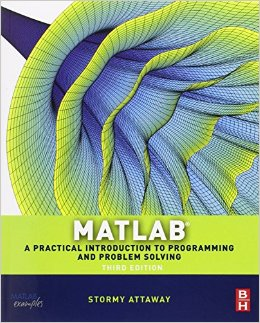
\includegraphics[width=0.8\linewidth]{matlab_stormy}
\end{center}
\end{marginfigure}

\section{Námsmat, einkunnir og próf}
\subsection{Fyrirlestraræfingar}
\label{sec:lecture-exercises}
Fyrirlestraræfingar eru í hverjum föstudagsfyrirlestri. Vægi þeirra er 10\% af lokaeinkunn. Þátttaka í $n$ fyrirlestraræfingum gefur hluteinkunnina $n$, að hámarki 10.

Tenglar á fyrirlestraræfingar verða gerðir aðgengilegir í hverri viku. Fyrirlestraræfingarnar verða nafni sínu samkvæmt hannaðar til að vera leystar í fyrirlestrartímunum sjálfum, en miðað verður við að hver þeirra verði opin í um það bil sólarhring.
\subsection{Skilaverkefni}
Vikuleg verkefnaskil eru í námskeiðinu. Meðaleinkunn 10 bestu skilaverkefnanna er 20\% af lokaeinkunn. Verkefnunum skal skila á Gradescope.com (sjá \nameref{sec:tools}). Ekki er tekið við seinum skilum.

Nauðsynlegt er að skila fjórum af fyrstu sex skilaverkefnunum til að öðlast próftökurétt.
\subsection{Próf}
Vægi lokaprófs er 70\% af lokaeinkunn. Leyfilegt verður að taka með eitt blað af glósum (skrifað á báðar hliðar) í lokapróf.

Lágmarkseinkunn er 5. Nauðsynlegt er að ná lágmarkseinkunn á lokaprófi sem og í námskeiðinu sem heild til að standast námskeiðið. 

Ekki er miðmisserispróf í námskeiðinu.
\section{Kennslutól}
\label{sec:tools}
Vefkennslutól verða notað eftir föngum. Mælt er með að nemendur skrái sig inn á eftirfarandi þjónustur sem allra fyrst:
\begin{itemize}
 \item \href{piazza.com/hi.is/fall2017/tl105g/home}{Piazza}\footnote{\url{piazza.com/hi.is/fall2017/tl105g/home}} er fyrirspurnavefurinn sem notaður er í námskeiðinu. Skráningin í námskeiðið á að vera sjálfvirk, en hafi það misfarist á að vera hægt að skrá sig handvirkt. Allar spurningar sem snúa að námskeiðinu ættu að fara inn á Piazza frekar en í tölvupóst.
 \item \href{https://gradescope.com/courses/8909}{Gradescope.com}\footnote{\url{gradescope.com/courses/8909}} er vefkerfið sem notað er til að taka við skilaverkefnum. Nemendur þurfa að skrá sig sjálfir á þennan vef. Aðgangskóði námskeiðsins er \texttt{9P7YGM}. Mikilvægt er að skrá sig á Gradescope með fullu nafni (íslenskir stafir eru leyfilegir) og með því að nota HÍ-netfang. Kerfið tekur við \texttt{.pdf} skrám.
\end{itemize}
Fyrir utan vefkennslutól er nauðsynlegt að nemendur setji upp þýðanda fyrir Java ásamt viðeigandi ritli á eigin tölvu eða útvegi sér aðgang að slíkri vél.

\section{Undanþágur og sérúrræði}
\href{http://nshi.hi.is/}{Náms- og starfsráðgjöf HÍ}\footnote{\url{nshi.hi.is}} hefur milligöngu um öll sérúrræði.

\end{document}